\documentclass{../../text-style}

\texttitle{Лекция 6: Планирование проекта}

\begin{document}

\maketitle
\thispagestyle{empty}

\attribution{сделано с активным использованием материалов Тимофея Александровича Брыксина, бывшего доцента кафедры системного программирования СПбГУ}

\section{Задача планирования}

Предположим, мы проанализировали требования, определили границы проекта, определили ключевых заинтересованных лиц (стейкхолдеров), разделили между ними ответственность, создали план коммуникаций и проделали всю прочую работу, необходимую перед стартом проекта. Однако у вас пока нет команды разработчиков, и перед тем, как её формировать, нужен план.

После предыдущего рассказа про Scrum может показаться, что ни план, ни архитектура современному проекту не нужны, мы просто формируем Scrum-команду, закидываем в бэклог пользовательские истории, и доверяем команде вести разработку. К сожалению, не всё так просто, потому что чтобы Scrum-команда появилась, нужны деньги на её зарплату, а для этого надо согласовать контракт с заказчиком (или, если это продуктовая разработка, согласовать параметры проекта с руководством компании). А для этого надо назвать цену и сроки, либо проекта в целом, либо ключевых этапов (помним, что в современном мире разработка программного обеспечения в большинстве случаев деятельность, а не проект). А для этого нужен план~--- с календарными сроками, исполнителями и финансовыми потоками.

В целом при планировании надо ответить на ряд ключевых вопросов:

\begin{enumerate}
    \item Что мы делаем? На этот вопрос отвечают требования, без требований планировать невозможно.
    \item Почему и зачем мы это делаем? На этот вопрос отвечают бизнес-требования и бизнес-цели проекта, их надо обязательно иметь в виду при планировании, чтобы не делать \enquote{чтоб было}.
    \item Когда? План прежде всего про календарные сроки, как проекта в целом, так и ключевых этапов проекта.
    \item Как? Технические детали реализации при планировании не рассматриваются, но методологию, общую архитектуру и иногда даже технологический стек стоит зафиксировать при планировании.
    \item Где? Кто? Ресурсы на разработку включают в себя команду (команды) разработчиков, вспомогательный персонал, также и помещения, и оборудование и т.п.
\end{enumerate}

Общая схема деятельности по планированию выглядит примерно вот так:

\begin{center}
    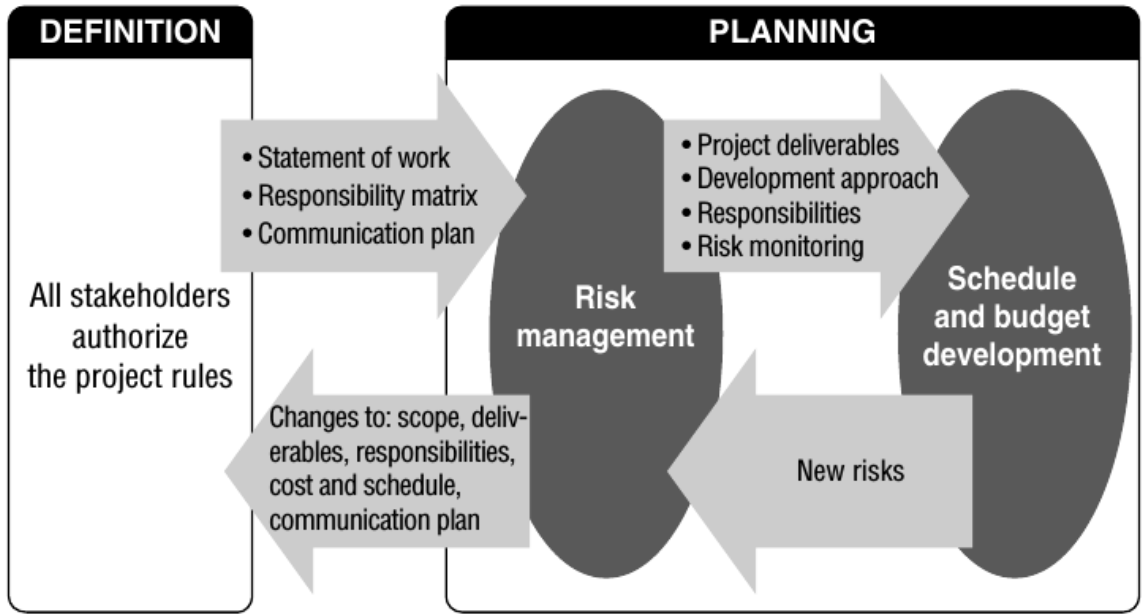
\includegraphics[width=0.7\textwidth]{planning.png}
\end{center}

Начинается всё с фазы определения проекта, на которой формулируется \enquote{statement of work} (у нас это называлось \enquote{документ об образе и границах системы}), где кратко описаны бизнес-цели и основные~требования проекта. Также на этой фазе создаётся ряд вспомогательных документов, если в них есть потребность~--- матрица ответственностей (за какой род деятельности какое заинтересованное лицо отвечает), план коммуникаций (кто когда и в какой форме должен кому что сообщать). 

Далее собственно фаза планирования, состоящая из двух крупных деятельностей --- оценки рисков и собственно составления графика работ (включая финансовые аспекты). Деятельность эта циклична, в ходе создания графика могут быть идентифицированы новые риски, которые могут привести к изменениям графика и т.д. Даже определение проекта может поменяться~--- например, мы поняли, что никак не уложимся в сроки с таким набором функциональности, надо урезать масштаб.

Определение проекта и требования мы уже обсудили на одной из предыдущих лекций, теперь поговорим подробнее о деятельности при планировании.

\section{Управление рисками}

Риски~--- это любые неприятные события, которые могут случиться по ходу проекта. Как правило, они разделяются на \enquote{известное неизвестное} и \enquote{неизвестное неизвестное}. Под \enquote{известным неизвестным} понимаются события, суть которых нам известна, однако неизвестно, произойдут они или нет. Такими рисками можно управлять, о чём мы поговорим далее. Под \enquote{неизвестным неизвестным} понимаются события, суть которых неизвестна, как и неизвестно, произойдут они или нет. С такими рисками бороться нельзя, как правило на них закладывают дополнительные ресурсы и надеются, что их хватит.

Само понятие управления рисками~--- это систематическая работа по выявлению рисков, их классификации и их устранению. Чрезвычайно важно здесь то, что эта работа систематическая: чем систематичнее ваш подход к рискам, тем лучше вы можете их контролировать. И когда что-то плохое случится, у вас уже будет заготовлен план противодействия.

Можно даже сказать, что управление рисками~--- основная работа менеджера. Причём на стадии планирования детальное планирование проекта и управления рисками идут рука об руку. Вы начинаете планировать новую задачу, выявляете риски этой задачи, определяете стратегию их устранения (о чём далее) и ставите задачу в план. То есть каждая задача при планировании должны быть оценена не только с точки зрения ресурсов, графика и т.д., но и с точки зрения возможных рисков.

Теперь пошагово разберем процесс управления рисками:

\begin{center}
    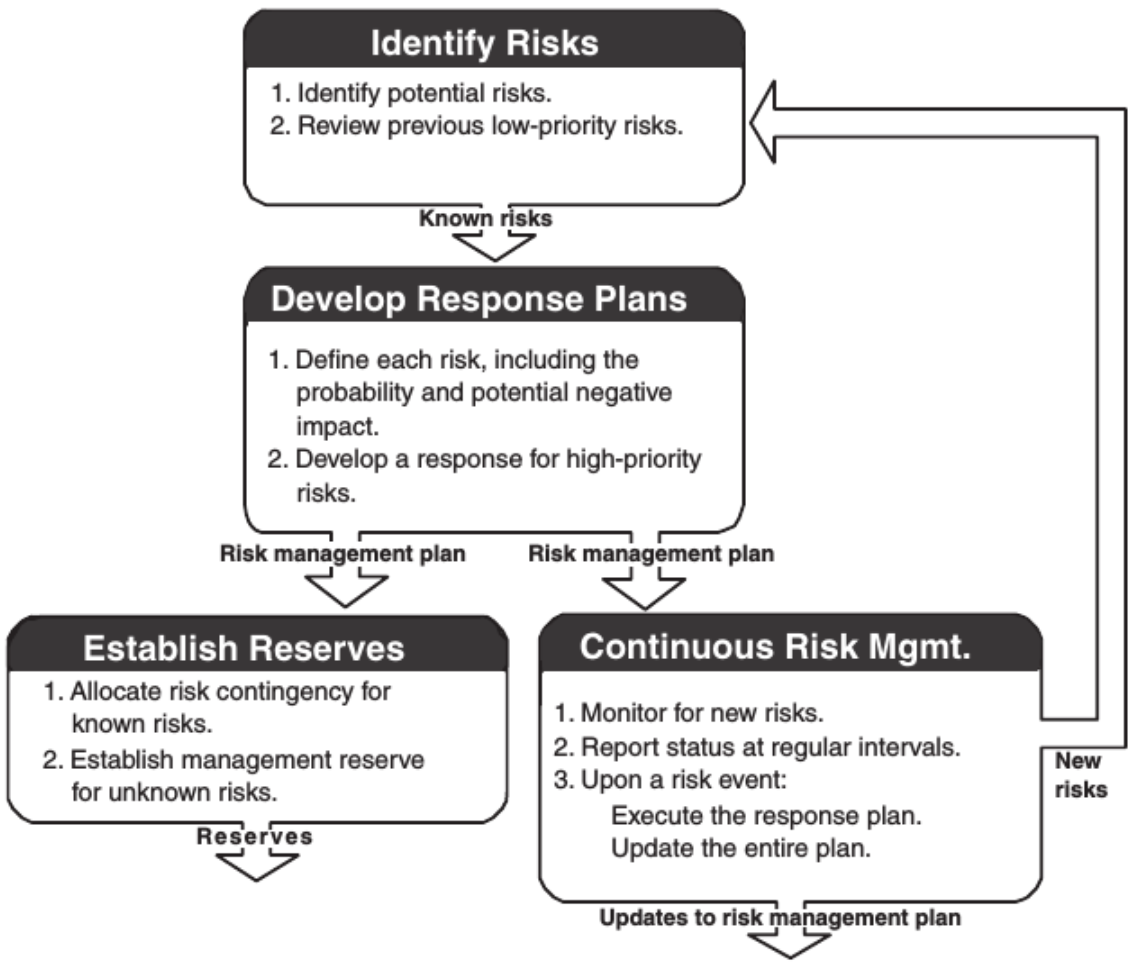
\includegraphics[width=0.7\textwidth]{riskManagementLoop.png}
\end{center}

\subsection{Распознавание риска}

На первой стадии управления рисками их необходимо идентифицировать. Для этого можно использовать разные методы, начиная от опроса стейкхолдеров и заканчивая привлечением статистических данных.

При опросе стейкхолдеров менеджер собирает их мнения относительно предполагаемых рисков, после чего анализирует полученную информацию. Менеджер выявляет возможные риски, группирует их по степени важности и вероятности и удаляет повторения. Данный анализ можно также проводить не через интервьюирование, а через мозговые штурмы. Тут важно записывать вообще всё, что только приходит в голову: потом риски можно будет приоритизировать и отбросить совсем уж маловероятные.

Другой подход~--- использовать профиль риска. В случае, если в компании производились похожие проекты, по ним должны были быть составлены специальные опросники, выявляющие наиболее часто встречающиеся в проектах такого типа риски~--- профили рисков. Используя их, вы можете выявить часть рисков. По окончании проекта предполагается, что вы также обновите профили риска новой информацией, полученной из данного проекта.

Можно использовать прошлый опыт и напрямую. Поднимите в архивах документацию по прошлым проектам такого типа. Графики, составленные их менеджерами, и реальные графики исполнения проектов дадут ценную информацию относительного того, что может пойти не так.

Наконец, часть рисков вы обнаружите прямо в ходе планирования. Просто отмечайте те задачи, которые трудно спланировать по времени и/или бюджету. Почти наверняка они содержат тот или иной фактор риска.

После того, как вы выявили риск, опишите его. Укажите условия при которых он может произойти и последствия, которые он повлечет. Удостоверьтесь, что из вашего описания ясно, в чём состоит риск, каковы его последствия, можно ли его избежать, и, если можно, то каких ресурсов это потребует. Помните, что чем детальнее вы определите риски и возможные последствия, тем лучше вы сможете риском управлять. Поэтому, данной части стоит уделить особое внимание.

К примеру, описание \enquote{В проекте нам придётся работать с технологией, с которой ни у кого из разработчиков нет опыта работы} довольно плохое. Понятно, что это риск, но как с ним бороться, по описанию даже предположить сложно. Его можно было записать иначе: \enquote{Заказчик требует интеграцию нашего приложения с его информационными системами по протоколу X, с которым в команде никто ранее не работал}. Такое описание более чётко описывает проблему и даёт возможность рассматривать варианты её решения.

Постарайтесь назначить риску некоторую вероятность. Определить её можно, исходя из статистических данных или из опыта. К сожалению, трудно формализовать процесс вычисления вероятности риска. В случае, если невозможно произвести более или менее строгую количественную оценку, можно произвести субъективную качественную оценку. Это менее точный вариант, однако это лучше, чем не оценивать вероятность риска вовсе. Привлекайте к оценке экспертов в этой области, человек без понимания ситуации даст гораздо менее надёжную оценку.

\subsection{Выработка стратегии противодействия}

При разработке стратегии противодействия нужно учитывать как вероятности риска, так и тяжесть его последствий. Если последствия и вероятность оценены количественно, то можно перемножить их и получить некоторую абсолютную величину опасности риска. В случае, если оценки производились качественно, можно использовать квадрат рисков.

\begin{center}
    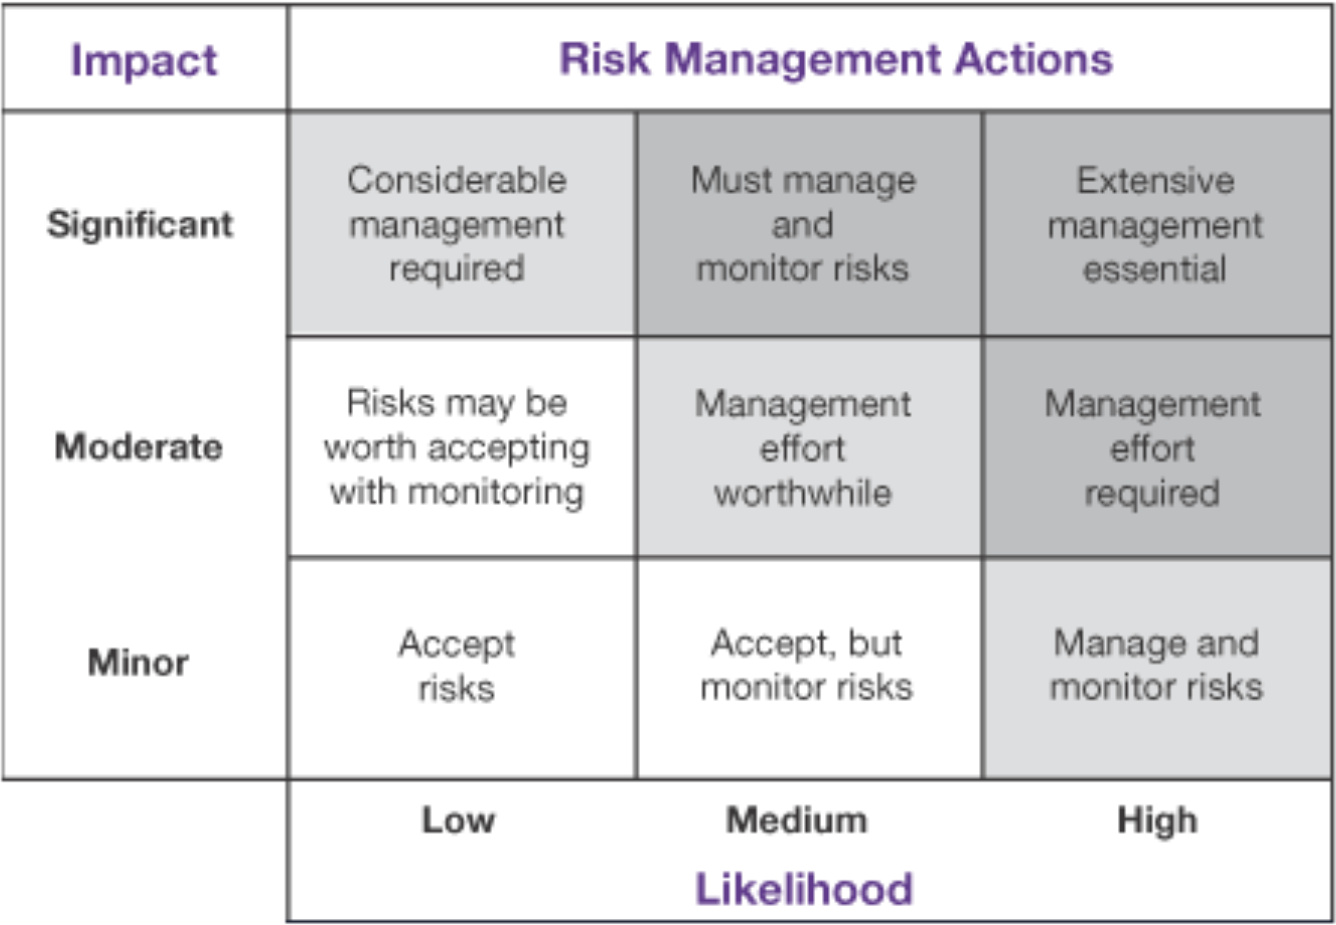
\includegraphics[width=0.6\textwidth]{riskMatrix.png}
\end{center}

Чем ближе риск к правому верхнему углу, тем риск \enquote{опаснее}, чем ближе к левому нижнем, тем он более \enquote{безопасен}.

Классифицировав некоторым образом риск по его опасности, можно применить к нему одну из стратегий противодействия рискам.

\emph{Принять риск.} Вы понимаете риск, его последствия, и решаете его принять, то есть не производить никаких активных действий по его устранению. Такая стратегия, как правило, применяется либо если риск находится в нижнем левом угле квадрата, либо если затраты на противодействие ему больше затрат на устранение последствий (и при этом они вписываются в бюджет).

\emph{Избежать риска.} Вы понимаете риск и решаете отказаться от реализации части системы, порождающей его. Как правило, такая стратегия применяется, если риск вероятен, его последствия велики, а предотвратить его стоит излишне дорого. Но тут нужно быть осторожным, поскольку велика вероятность лишить свой продукт одного из конкурентных преимуществ. Как правило, чем больше риск реализации чего-то, тем больше пользы это что-то приносит.

\emph{Переложить риск.} Вы понимаете риск и решаете предоставить возможность разобраться с ним приглашенному специалисту или вообще отдать эту задачу на аутсорсинг. Нужно понимать, что при этом риск и его последствия не исчезают, но контролировать его вы больше не можете. Это уже не ваша ответственность, но всё ещё ваша головная боль. К тому же, вы получаете новые риски взаимодействия с экспертами/субподрядчиками.

\emph{Смягчить риск.} Вы понимаете риск и решаете провести сейчас некоторые дополнительные работы, смягчающие его возможные последствия (к примеру, если есть риск, что команда не успеет разобраться в новой технологии, то вы можете пригласить эксперта по ней, чтобы он провел мастер-класс).

\emph{Отслеживать риск.} Вы понимаете риск и решаете отслеживать вероятность его возникновения. В случае, если вероятность возникновения риска достигнет какого-то критического значения, вы начнете предпринимать активные действия по его предотвращению. Однако, при отслеживании риска важно понимать, насколько мы в состоянии адекватно отслеживать и предсказывать его появление. Если риск из вероятного превратится в наступивший в течении пары секунд, вариант с отслеживанием не для вас. Но и если риск будет медленно наступать в течение пары лет, у вас должен быть чёткий критерий того, что риск уже случился, и нужно начинать ему противодействовать. Ситуация будет напоминать историю про лягушку, сварившуюся в кастрюле\footnote{\url{https://ru.wikipedia.org/wiki/Лягушка_в_кипятке}}.

Результаты анализа рисков и построения стратегий противодействия имеет смысл организовать в таблицу, в которой указываются не только риски и их приоритетность, но и ответственные и статус самого риска.

\subsection{Создание резервного фонда}

Противодействие рискам требует бюджета. Очень маловероятно, что получится сформировать такой резервный фонд, которые будет покрывать все описанные риски вообще (крайне маловероятно, что сразу случится вообще всё плохое, что только может), поэтому чаще всего компромисс достигается путём анализа, предположений и переговоров. Как правило, вычисляют размер этого фонда следующим образом: отбирается наиболее вероятная часть рисков, вероятность этих рисков умножается на стоимость противодействия им и складывается, к результирующей сумма прибавляется 5-30\% от бюджета проекта на неизвестные риски. Процент на неизвестные риски зависит от специфики проекта, опыта компании, команды и лично менеджера. 

Проблема с резервным фондом состоит в том, что если вы заложите на риски слишком много, итоговая стоимость проекта вырастет настолько, что станет неприемлема для заказчика (или просто выше, чем у конкурентов). А если слишком мало~--- то в случае, если риски всё-таки реализуются, компенсировать их будет нечем и мы превысим сроки или бюджет проекта, что принесёт нам потерю прибыли, репутационные потери и, возможно, неустойку. Однако заложить ровно столько, сколько надо, мы не можем, поскольку не можем все риски идентифицировать. Всё, как обычно, зависит от интуиции и опыта менеджера.

\subsection{Непрерывное управление рисками}

Но на этом всё не заканчивается. После старта проекта менеджер должен постоянно отслеживать риски, оценивать их и предлагать стратегии противодействия. Соответственно, задачей менеджера становится:

\begin{itemize}
    \item отслеживать текущие риски;
    \item выявлять новые риски, оценивать их и предлагать стратегии противодействия;
    \item проводить регулярную полную переоценку рисков на предопределенных стадиях проекта (например, завершение прототипа, выход нового релиза и т.д.). Собственно, эту информацию удобно отображать в колонке \enquote{статус} в предыдущей таблице.
\end{itemize}

Непрерывное управление рисками гарантирует, что менеджер всегда будет в курсе текущих рисков проекта и сможет грамотно на них отреагировать.

\section{Декомпозиция проекта}

Следующей стадией планирования является декомпозиция проекта. Невозможно анализировать сложный проект, рассматривая его как целое~--- как правило требуется сначала разбить его на части/подзадачи, то есть создать Work Breakdown Structure (WBS), и лишь потом анализировать.

Достаточно маленькую подзадачу уже можно проанализировать и спланировать: определить затраты ресурсов, риски исполнения и роли стейкхолдеров, которые должны будут принять участие в реализации задачи. С помощью декомпозиции можно получить достаточно точный и детализированный план выполнения проекта.

Представлять разбиение задач можно в графической или текстовой форме. Графическая более наглядна, но может быть неудобна в использовании при большом количестве задач. Например, она может выглядеть так:

\begin{center}
    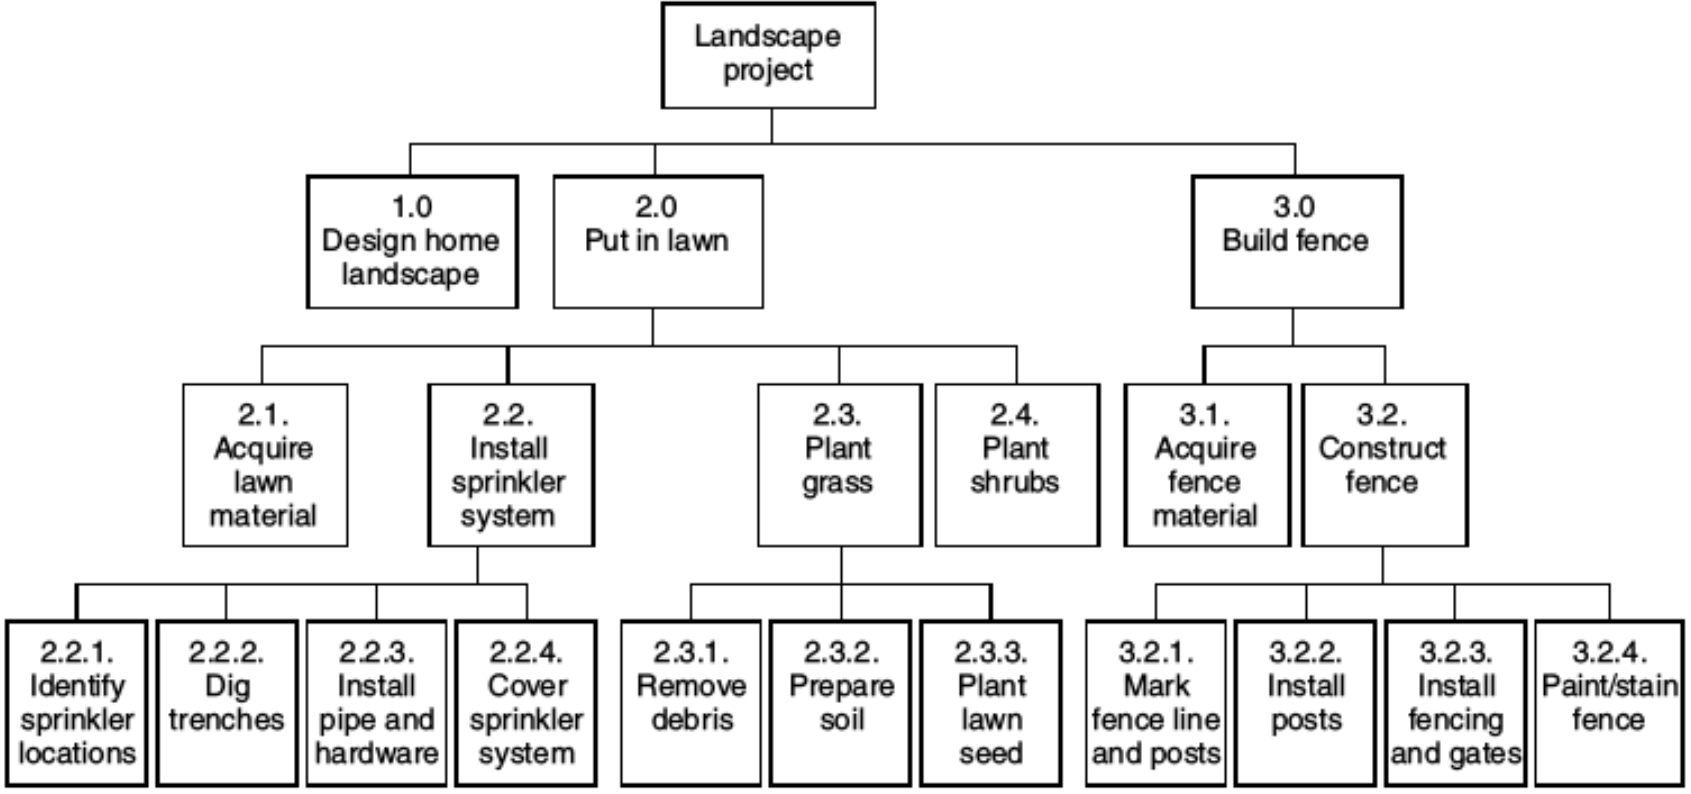
\includegraphics[width=\textwidth]{wbsExample.png}
\end{center}

Или вот так:

\begin{center}
    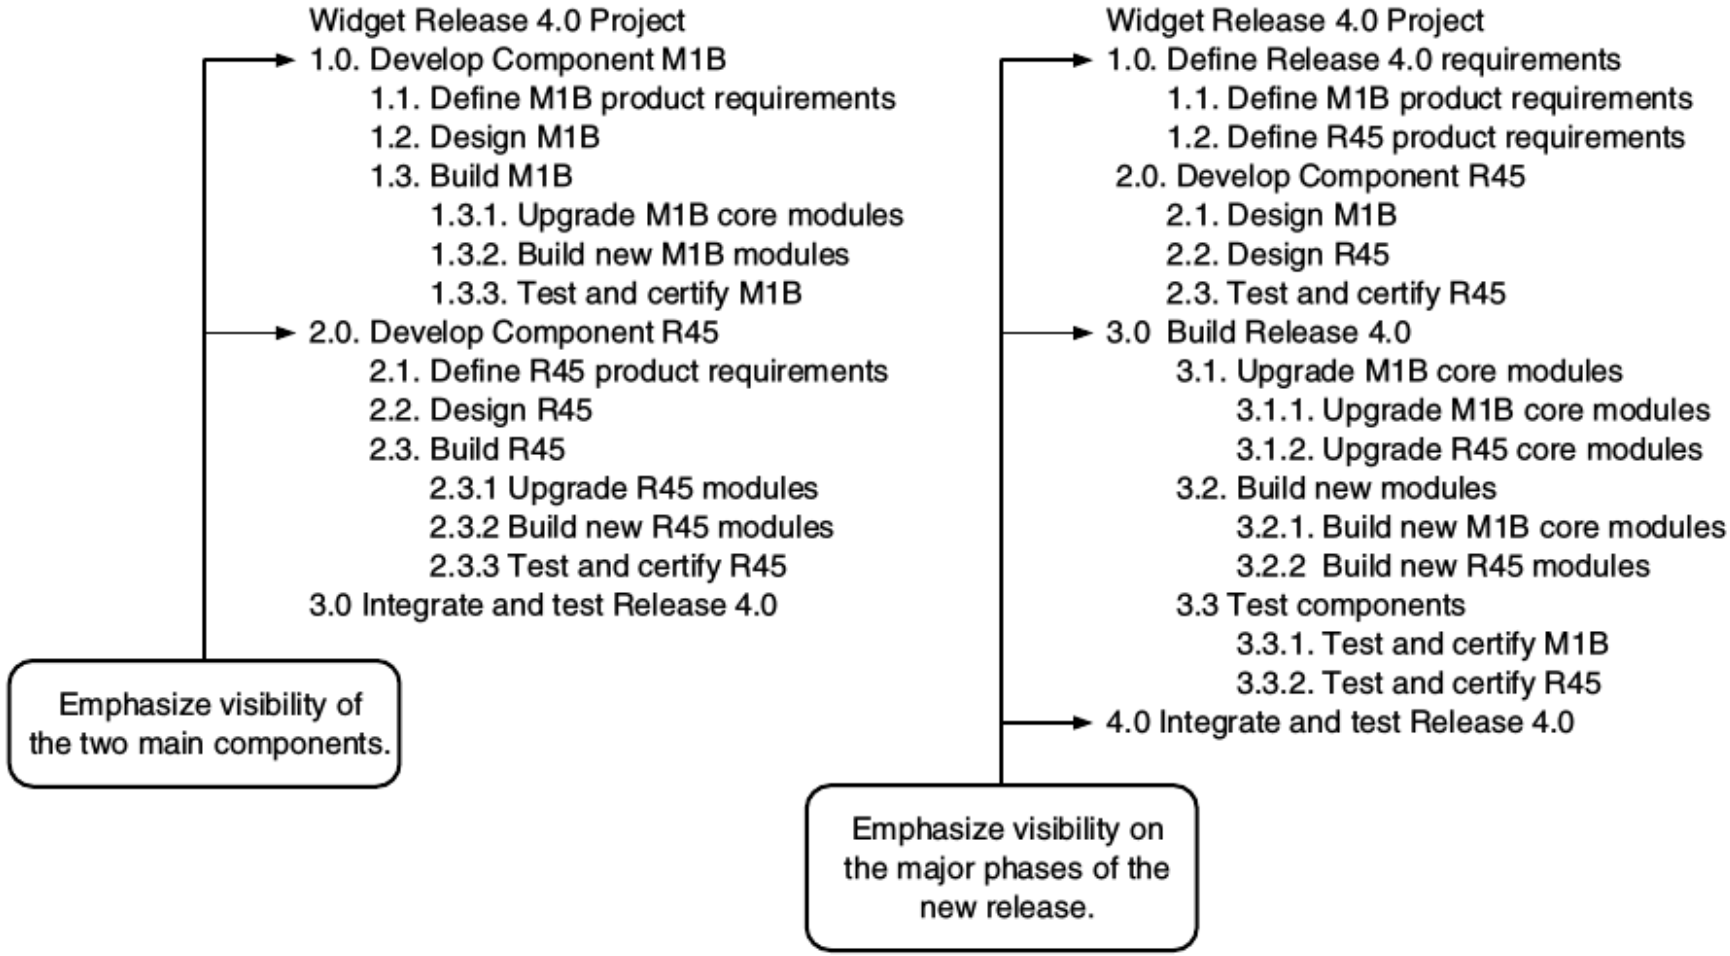
\includegraphics[width=0.9\textwidth]{wbsExample2.png}
\end{center}

Качественное дерево задач можно использовать для иллюстрации границ проекта и для отслеживания прогресса. В дальнейшем дерево декомпозиции будет основой для построения плана проекта и оценки его длительности и необходимого бюджета.

\subsection{Методы декомпозиции}

Декомпозицию можно делать по-разному. Во-первых, это может быть нисходящая декомпозиция: вы берёте абстрактную задачу (например, сделать такой-то продукт) и разбиваете её до тех пор, пока не получите вполне конкретные задачи по производству конкретных частей данного продукта. Эти задачи должны быть настолько малы, что вы легко можете их анализировать, оценивать и понимаете процесс исполнения этих задач (если вы не понимаете процесс, который стоит за этой задачей, то привлеките экспертов). Итоговые задачи можно переупорядочить и получить общий процесс выполнения проекта. Другой подход~--- идти от высокоуровневых видов деятельности, которые нужно совершить (см. левый и правый вариант списка на рисунке выше), и дальше разбивать их на более мелкие работы.

Во-вторых, восходящая: вы рассматриваете конкретные задачи по созданию частей продукта и уже из них собираете сам продукт.

Заметим, что не всякая декомпозиция должна быть полной. Каждой команде или стейкхолдеру проекта на самом деле требуется некоторая проекция на декомпозицию~--- её модель, скрывающая все ненужные детали и подчеркивающая важные. Важно это понимать и не слать на каждый запрос плана проекта полную схему, а предоставлять лишь то, что действительно нужно.

\subsection{Критерии хорошей декомпозиции}

Если декомпозиция нисходящая, то каждая подзадача должна действительно быть подмножеством объемлющей задачи. В случае, если это не так, то декомпозиция просто неверна. Также все дети задачи в сумме должны давать саму задачу. Это тоже обязательное условие корректности декомпозиции (так называемое \enquote{правило ста процентов}), дальше мы будем использовать этот факт при оценке задач.

Описание задачи должно явно содержать глагол, который определяет ключевую деятельность и явное существительное, которая определяет главный артефакт. \enquote{Протестировать модуль A}, \enquote{Реализовать модуль B}, \enquote{Спроектировать модуль C}. То есть такие задачи, которые потом можно будет поместить в таск-трекер и раздавать членам команды. Примеры плохих задач: \enquote{Провести исследование}, \enquote{База данных}.

\subsection{Размеры конечных задач}

Определение размеров конечных задач~--- вопрос чрезвычайно субъективный. Размеры задач зависят от вашего опыта в планировании, размеров проекта и ресурсов, выделенных для планирования проекта. Тем не менее, есть некоторые общие рекомендации.

Есть известное \enquote{правило 8/80}: согласно ему, работа над задачей должна занимать не менее восьми и более восьмидесяти часов.

В случае, если в вашей организации есть некоторые установленные периоды отчетности (например, еженедельные доклады о статусе проекта), то удобно, чтобы задачи занимали не более, чем два отчёта. В таких случаях вы не окажетесь в ситуации, когда на докладе о статусе разработчик будет говорить, что сделано 37\%. Задача будет либо сделана, либо нет.

Также при выборе размеров конечных задач стоит руководствоваться здравым смыслом. При размере задач в 15 человеко-минут спланировать проект будет стоить чрезвычайно дорого, а сам процесс будет очень неэффективен из-за постоянного микроменеджмента. Та же проблема и со слишком большими задачами.

К тому же, при изменении целей или деталей проекта некоторые участки дерева задач могут оказаться больше неактуальными. Так что при декомпозиции стоит соблюдать разумный баланс в объёме задач в листьях дерева.

\subsection{Критерии SMART}

Есть известный набор критериев, которым должна удовлетворять задача в проекте, называющийся \enquote{критерии SMART}.

\begin{itemize}
    \item Specific~--- задача должна быть конкретной и однозначно пониматься всеми участниками.
    \item Measurable~--- задача должна быть измеримой, желательно иметь чёткие булевые или числовые критерии того, насколько задача сделана.
    \item Achievable~--- задача должна быть достижимой: она должна быть осуществимой в принципе, у неё должны быть реалистичные сроки (пример нарушения этого принципа из жизни: \enquote{прошу к завтра до 12:00 представить предложения по концепции стратегии развития IT-образования в Российской Федерации}), на неё должно быть в принципе возможно выделить требуемые ресурсы (материальные и трудовые).
    \item Relevant~--- задача должна быть значимой и укладываться в общую стратегию проекта. Необязательные задачи можно просто не делать, а раз что-то можно не делать, то делать это и не нужно.
    \item Time bound~--- задача должна быть ограниченной по времени. Текущую деятельность не планируем и не оцениваем, она будет просто влиять на продуктивность. Есть хорошее правило \enquote{8/80}, которое говорит, что \enquote{листовая} задача в Work Breakdown Structure должна оцениваться не менее чем в 8 часов и не более чем в 80 часов. Слишком мелкая декомпозиция усложняет процесс планирования и всё равно оказывается бесполезной по ходу работы (особенно если у вас agile-проект), слишком крупная сильно загрубляет оценку и  усложняет контроль.
\end{itemize}

\section{Построение графика работ}

Планирование проекта предполагает множество взаимосвязанных итераций, итогом которых выступает единый сводный план. Рассмотрим основные задачи планирования (первые три из них мы уже рассмотрели, остальные рассмотрим ниже).

\begin{enumerate}
    \item \emph{Определение целей проекта и требований.} В первую очередь необходимо понять, \enquote{что вы будете производить}, прежде чем решать, \enquote{как это производить}. Вы уточняете и детализируете цели и результаты проекта.
    \item \emph{Анализ рисков.} На этом этапе вы выявляете препятствия, которые могут возникнуть в ходе реализации проекта, оцениваете их, а затем определяете варианты действий по их устранению.
    \item \emph{Декомпозиция проекта.} Невозможно анализировать сложную систему, рассматривая ее как единое целое. Поэтому, как правило, требуется сначала разбить ее на части (подсистемы) и лишь потом проводить анализ.
    \item \emph{Выявление зависимостей между задачами.} При планировании задач необходимо учитывать взаимосвязи между ними. Например, вы не можете начать писать документацию, пока не будут разработаны компоненты системы. В свою очередь проект не будет принят заказчиком, пока не будет написана документация. Поэтому необходимо определить, какие связи есть между задачами, в каком порядке их нужно выстроить.
    \item \emph{Оценка задач.} Для каждой задачи определяются объем работы и ее длительность, которая измеряется в человеко-часах/-днях/-неделях.
    \item \emph{Создание и оценка плана работ.} После того, как вы разбили ваш проект на задачи, установили последовательность их выполнения и оценили каждую из них, вы составляете план. Здесь уже вычисляются сроки выполнения всего проекта, указываются запланированные даты начала и завершения. Но следует учитывать, что первоначальный план, скорее всего, не будет соответствовать имеющимся ограничениям по производственным ресурсам, времени или каким-нибудь другим параметрам. Поэтому есть еще пункт 7.
    \item \emph{Распределение и оптимизация ресурсов.} Планирование~--- это итеративный процесс. С первого раза его очень сложно сделать правильно, поэтому эта стадия предполагает серьезную корректировку всего графика, который был построен до этого. Задачи перепланируются с целью оптимизации распределения людей и ресурсов, используемых в проекте. Вы получаете новую информацию, основываясь на которой можете более точно спланировать вашу деятельность.
\end{enumerate}

Таким образом, эти шаги генерируют довольно много информации, необходимой для понимания того, как будет выполняться проект. Эта работа сильно итеративная, с первого раза вряд ли сразу получится получить хороший план.

\subsection{Матрица зависимостей}

\begin{center}
    \begin{tabularx}{\textwidth} { 
        | >{\centering\arraybackslash}X 
        | >{\centering\arraybackslash}X 
        | >{\centering\arraybackslash}X | }
        \hline
        Операция                                  & Непосредственно предшествующие операции & Длительность \\
        \hline
        A. Установка компьютеров                  &~---                                     & 1            \\
        \hline
        B. Протяжка сети                          &~---                                     & 2            \\
        \hline
        C. Настройка сети                         & A, B                                    & 3            \\
        \hline
        D. Установка программного обеспечения     & C                                       & 1            \\
        \hline
        E. Разработка регламента использования ПО &~---                                     & 4            \\
        \hline
        F. Обучение пользователей                 & D, E                                    & 3            \\
        \hline
    \end{tabularx}
\end{center}

После того как вы определили задачи проекта, необходимо определить связи между ними. Зависимости между задачами влияют на даты планируемого начала или завершения задач. Наиболее распространенный тип связи~--- это когда работа B не может начаться раньше, чем закончится работа А. Например, задача \enquote{интегрировать модуль Х} не может начаться, пока не завершится задача \enquote{реализовать модуль Х}.

Матрица зависимостей представляет собой простой, но эффективный метод обнаружения связей между задачами. Вы выписываете все задачи, нумеруете их каким-нибудь уникальным идентификатором и пишите, за какой задачей должна выполняться конкретная задача.

Но следует учитывать, что когда у вас есть большое количество задач и между ними сложные зависимости, то такая форма представления может оказаться ненаглядной. Чаще всего используют так называемый сетевой график.

\subsection{Сетевой график}

Сетевой график~--- это модель, отражающая зависимость и последовательность выполнения задач. Этот график передает ту же самую информацию, что и матрица зависимостей, но он более наглядный: на нём гораздо более явны потенциальные проблемы и возможности для их решения. Например, вначале часто удобно бывает построить таблицу, а потом по ней уже график.

Основными параметрами сетевого графика являются работа и событие. Под работой подразумевается любой процесс, требующий затраты времени. Событие~--- это промежуточный или окончательный результат одной или нескольких работ, необходимый для начала других работ. Событие совершается после выполнения всех работ, входящих в него. Работу на сетевом графике изображают одной сплошной стрелкой. Продолжительность работы в единицах времени (часы/дни/недели) и наименование работ обычно пишут рядом со стрелкой. Каждое событие изображается кружком и нумеруется.

\begin{center}
    \begin{tikzpicture}
        [every path/.style={font=\ssmall}]

        \node[shape=circle,draw=black] (1) at (0,0) {1};
        \node[shape=circle,draw=black] (2) at (2.5,1.5) {2};
        \node[shape=circle,draw=black] (3) at (2.5,-1.5) {3};
        \node[shape=circle,draw=black] (4) at (5,0) {4};
        \node[shape=circle,draw=black] (5) at (8,0) {5};
        \node[shape=circle,draw=black] (6) at (11,0) {6} ;
        
        \path [->](1) edge node[align=center] {A. Установка компьютеров\\ \textit{1 день}} (2);
        \path [->](1) edge node[align=center] {B. Протяжка сети\\ \textit{2 дня}} (3);
        \path [->,dashed](3) edge node[] {} (2);
        \path [->](2) edge node[align=center] {C. Настройка сети\\ \textit{1 день}} (4);
        \path [->](4) edge node[align=center,below=5pt] {D. Установка программного\\ обеспечения\\ \textit{1 день}} (5);
        \path [->](5) edge node[align=center,below=5pt] {F. Обучение\\ пользователей\\ \textit{1 день}} (6);
        \path [->](1) edge[bend right=70] node[align=center,below] {E. Разработка регламента\\использования ПО\\ \textit{1 день}} (5);
    \end{tikzpicture}
\end{center}

Здесь есть два важных момента.

\begin{enumerate}
    \item Задачи, которые попадают в этот график~--- это те самые задачи, которые вы получили при декомпозиции, которые вы потом будете \enquote{делать руками}. Т.е. тут не пишутся задачи, которые находятся в промежуточных узлах и обобщают задачи уровня ниже. Сюда заносятся только те задачи, которые вы реально будете делать, которые вы будете оценивать, из которых будет строиться все состояние.
    \item Сетевой график должен отражать только зависимости между задачами. Не надо строить этот график, учитывая те ресурсы, которые у вас есть. Просто забудьте о них. Представьте, что у вас есть неограниченное число людей, денег и т.д. Изменение сетевых графиков из-за ограничений ресурсов является наиболее распространенной ошибкой при построении такого рода диаграмм. Тот факт, что не хватает людей или других ресурсов для одновременного выполнения нескольких задач, не имеет значения. Независимо от ресурсов, задачи все равно должны выполняться в том же порядке.
\end{enumerate}

\subsubsection{Основные правила разработки сетевого графика}

При разработке сетевого графика целесообразно придерживаться следующих правил:

\begin{itemize}
    \item Ни одна операция не может быть начата, пока все предшествующие связанные с ней операции не будут выполнены.
    \item Стрелки в сетевом графике отображают отношения предшествования и следования. На рисунке стрелки могут пересекаться.
    \item Каждая операция должна иметь свой собственный номер.
    \item Номер последующей операции должен быть больше номера любой предшествующей операции.
    \item Образование петель недопустимо (другими словами, не должно происходить зацикливания хода выполнения установленного набора операций).
    \item Условные переходы от одной операции к другой не допускаются (имеется в виду определение последовательности хода выполнения операций условиями типа: \enquote{Если будет достигнут успех, сделайте то-то...; если нет~--- ничего не предпринимайте}).
\end{itemize}

При включении любой операции в сетевой график необходимо определить для нее три отношения. Эти отношения могут быть определены в результате ответов на следующие три вопроса:

\begin{itemize}
    \item Какие операции должны быть завершены непосредственно перед этой операцией?
    \item Какие операции должны следовать непосредственно за этой операцией?
    \item Какие операции могут выполняться во время выполнения этой операции? Какие операции можно назвать параллельными данной?
\end{itemize}

\subsubsection{Внешние события и майлстоуны}

Часто на сетевом графике бывает удобно указывать также внешние для проекта события и ключевые точки (майлстоуны) проекта. Они не требуют никакого времени и не влияют на продолжительность путей в сетевом графике, однако часто удобны для синхронизации хода работ. К ним можно отнести точки начала и завершения работ, даты выпуска версий ПО, события получения денег от заказчика или что-то ещё.

\subsection{Оценка задач}

После того, как вы нарисовали такой график, выяснили, что от чего зависит, нужно каждую задачу аккуратно оценить. Оценивают их обычно по времени. Только необходимо понимать, что это не фактическое время выполнение задачи, а время от начала реализации этой задачи до получения конечного результата. Т.е. если вы сделали задачу за 20 мин, а потом запустили тесты, чтобы проверить, и они, например, идут два дня, то время выполнения данной задачи будет не 20 мин, как это ошибочно можно полагать, а 2 дня и 20 мин. Это очень важный момент, поэтому вы должны четко представлять, что является конечным результатом конкретной задачи.

Есть еще такое понятие, как объем работы, и это именно то, в чём скорее всего будут оценивать задачи технические специалисты. Для того, чтобы конвертировать объём работы в календарное время, вам нужно знать продуктивность людей, которые будут делать эту задачу. Есть очень простая формула:

$$\textup{Длительность работ} = \frac{\textup{Объём работ}}{\textup{Производительность}}$$

Но эту формулу очень сложно применять, поскольку, как правило, вы не знаете ни числитель, ни знаменатель. Вы, конечно, можете примерно прикинуть и то, и другое, но с погрешностью, и эта погрешность может оказаться довольно большой.

Все понимают, что разные программисты пишут код по-разному, с различной скоростью. И здесь нельзя просто взять и посчитать среднюю производительность. Представьте, что у вас есть четыре программиста, у первых двух высокая продуктивность, у вторых двух низкая. Вы посчитали среднюю производительность, и затем задача досталась одному из них. Если она попала первым двум программистам, то они сделают ее быстрее, а если она попала другим двум, они просто не успеют. Ну и не стоит забывать, что один и тот же человек работает с различной производительностью в разные дни. Это сильно усложняет точную оценку, но в некотором приближении пользоваться этим всё равно приходится. Тут многое зависит от того, насколько хорошо вы знаете свою команду, а команда знает проект, который вы планируете.

Ещё при конвертации объёма работ во время не стоит рассчитывать, что каждый разработчик будет стабильно выдавать вам по 8 часов продуктивной работы каждый день. Продуктивно писать код по 8 часов в день довольно сложно, разработчики так или иначе оказываются вовлечены в разные совещания, планирование и оценку, проектирование, да и просто могут помогать коллегам с их задачами. Правильные коэффициенты тут тоже выясняются обычно опытным путём и сильно зависят от конкретных людей и принятых процессов.

Отдельная сложность при планировании работы людей, занятых на нескольких проектах сразу. Сложность совмещения проектов заключается в переключении контекстов. Разработка ПО~--- крайне творческая задача, часто требующая серьёзного погружения в предметную область, имеющийся код и особенности задачи. Если человека постоянно дёргать туда-сюда между проектами и задачами, он просто большую часть времени будет тратить на переключение между ними, а на собственно решение задач будет оставаться гораздо меньше восьми часов в день. Ну и в чём-то схожая ситуация с людьми, занятыми не на полную ставку (разного рода стажёры и т.п.), им может приходиться тратить какое-то время на синхронизацию с тем, что было сделано другими членами команды в их отсутствие.

Вот некоторая статистика, которую авторы статьи Astromskis et al. Patterns of Developers Behaviour: A 1,000-hour Industrial Study, 2017 собрали по шестерым разработчикам одной компании, занимавшейся разработкой встроенного ПО на C++, наблюдая за их действиями более тысячи рабочих часов:

\begin{center}
    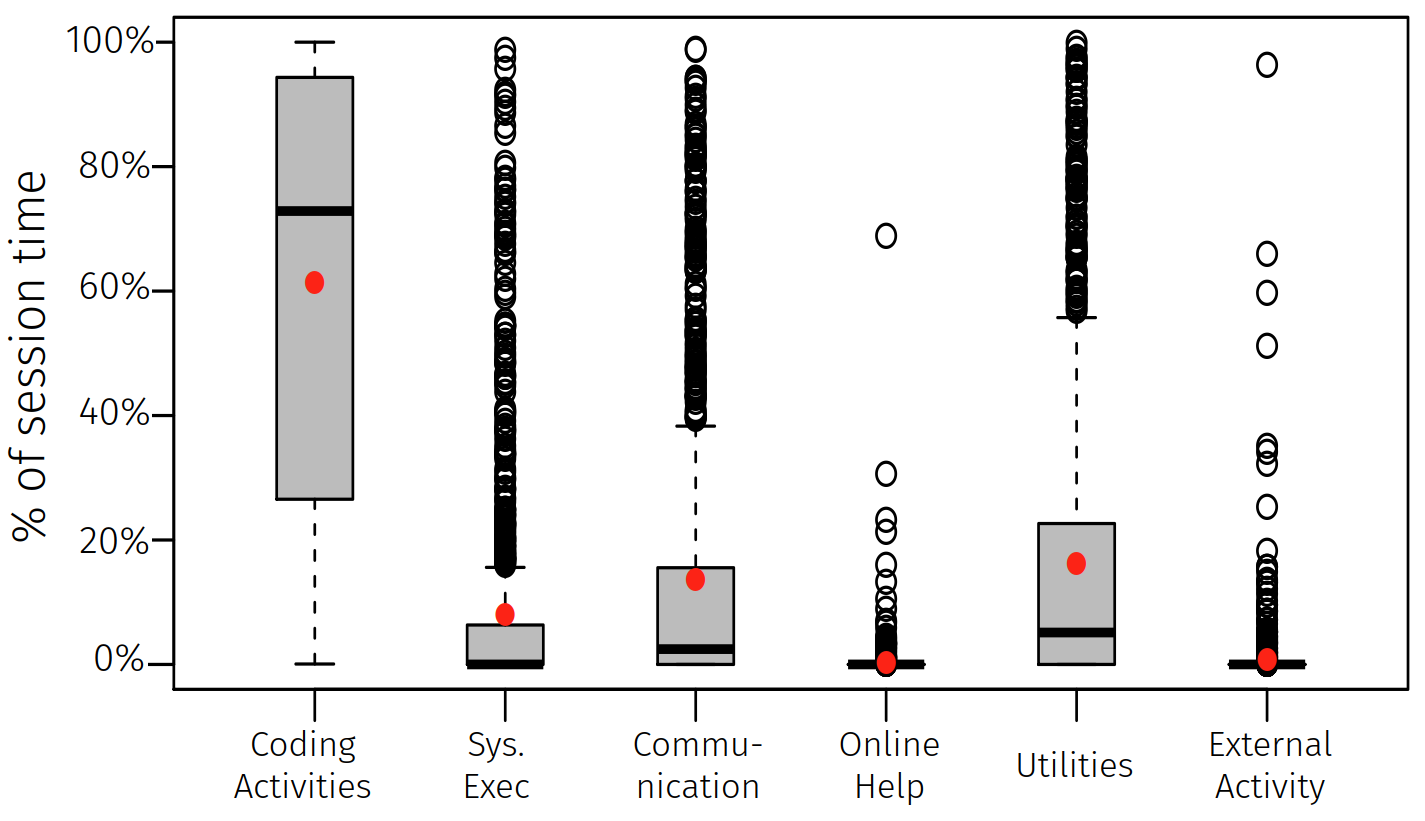
\includegraphics[width=0.95\textwidth]{timeSpentDuringWorkingSession.png}
    \attribution{Astromskis et al. Patterns of Developers Behaviour: A 1,000-hour Industrial Study, 2017}
\end{center}

Авторы разбили всю деятельность на работу с кодом (чтение или написание, не важно), запуск разрабатываемой системы, коммуникацию с коллегами (посредством мессенджеров, живое общение не входило), поиск информации в интернете, использование разного вспомогательного ПО, и деятельность, не относящуюся к работе. Статистика собиралась только во время рабочих сессий, то есть когда разработчик сидел за компьютером и что-то активно делал.

Выяснилось, что на собственно работу с кодом уходило порядка 60\% рабочего времени, 8\% на запуск системы (скорее всего, для тестирования), 16\% на вспомогательные инструменты (данные подготовить или что-то такое), 2\% (всего!) на поиск справки в интернете, 14\% на коммуникацию, 1\% на нерабочие активности (новости почитать, например). Статистику нельзя обобщать на все команды и все компании, но становится понятно, что даже то, что мы считаем плотной работой, на самом деле довольно сильно разбавлено вспомогательными процессами.

А если посмотреть на статистику по рабочему времени всего, а не только активной работы, станет ещё понятнее, почему человеко-день в 8 часов~--- это заведомый провал:

\begin{center}
    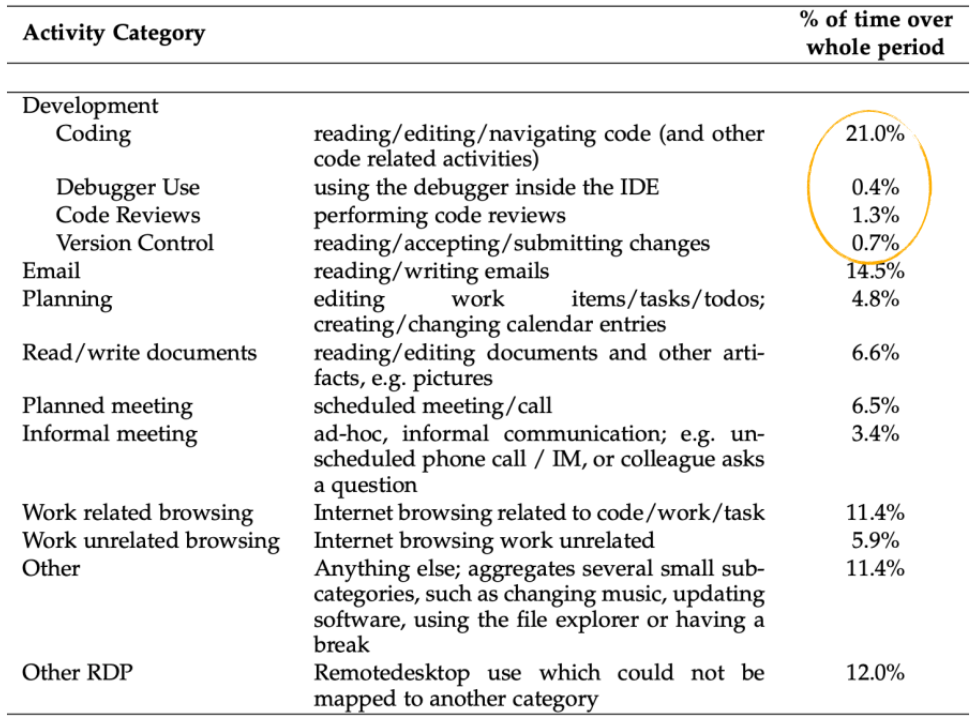
\includegraphics[width=0.7\textwidth]{timeSpentTotal.png}
    \attribution{Meyer et al. The work life of developers: Activities, switches and perceived productivity, 2017}
\end{center}

Причём это нормальная, честная и хорошая работа.

\subsection{Оценка графика работ}

Предположим, что вы как-то оценили все ваши задачи. Теперь вы хотите построить общий график и вычислить сроки выполнения всего проекта. Делается это на основе того же самого сетевого графика, только теперь он немного видоизменяется.

\begin{center}
    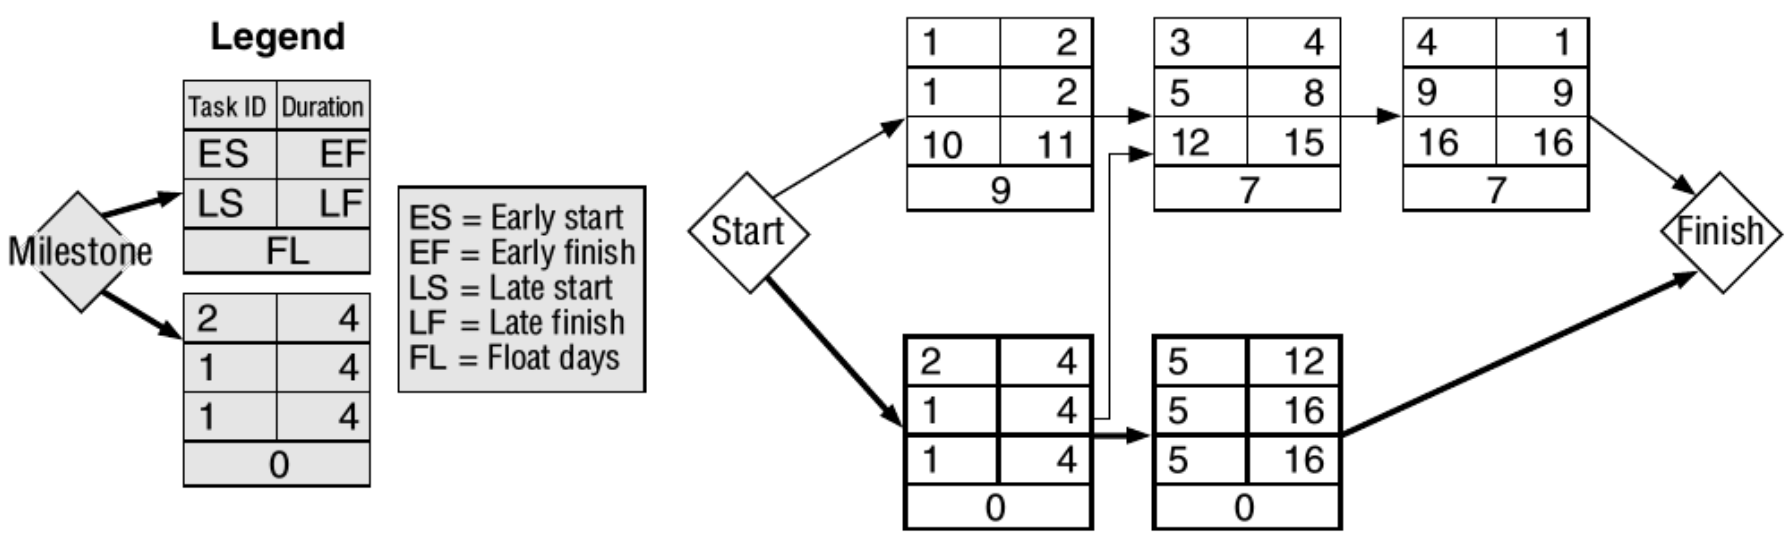
\includegraphics[width=0.95\textwidth]{graphEstimate.png}
\end{center}

По сути, справа нарисован сетевой график. Табличка слева~--- это легенда, которая просто показывает, что эти кубики значат. Здесь используются следующие понятия.

\begin{itemize}
    \item \emph{Раннее начало (Early start, ES)}~--- это самая ранняя дата, с которой может начаться задача. Т.е. эта величина показывает время, раньше которого задача не может быть начата.
    \item \emph{Раннее окончание (Early Finish, EF)} определяется суммой раннего начала и продолжительности рассматриваемой задачи.
    \item \emph{Позднее начало (Late Start, LS)}~--- это самая поздняя дата, когда задача может быть начата без задержки завершения проекта. Т.е. эта величина показывает время, позже которого задача не может быть начата без увеличения продолжительности всего проекта.
    \item \emph{Позднее окончание (Late Finish, LF)} вычисляется как сумма позднего начала и продолжительности рассматриваемой задачи.
\end{itemize}

Первая строчка элемента сетевого графика: слева идентификатор (номер задачи), а справа~--- длительность. Т.е. глядя на первый прямоугольник, вы понимаете: задача 1 длительностью в 2 единицы. Во второй/третьей строчке записываются раннее/позднее начало и раннее/позднее окончание.

Теперь о том, как это все вычислить. В самом начале у вас все ячейки пустые, кроме первой строки. Идентификатор задач и их длительность вы знаете.

\subsubsection{Шаг 1. Прямой проход}

Он называется так потому, что вычисления начинаются с исходного события и продолжаются до тех пор, пока не будет достигнуто завершающее событие. Прямой проход помогает вам определить раннее начало и раннее окончание для каждой задачи. Пойдем по порядку:

\begin{enumerate}
    \item Первая задача. Она занимает два дня. Значит, это первый и второй день. Следовательно, early start = 1, early finish = 2. Идем дальше в задачу 2.
    \item Вторая задача. Она ни от чего не зависит. Значит, ее можно начать выполнять сразу же (в первый день). Длительность = 4, поэтому early finish = 4.
    \item Третья задача. Она не может начаться раньше, чем завершится задача 2. Поэтому у нее early start = 5, early finish = 8.
\end{enumerate}

И так далее вы заполняете эти оптимистичные оценки.

\subsubsection{Шаг 2. Обратный проход}

Обратный проход  определяет позднее начало и позднее окончание. Цель обратного прохода~--- пройтись в обратном направлении от даты окончания проекта, чтобы определить, насколько поздно любая задача может начаться и завершиться, чтобы проект всё ещё уложился в срок, полученный при прямом проходе. Т.е. вы берете последнюю дату и смотрите: \enquote{если мы в этот момент все закончим, то когда должна начать выполняться последняя задача?}. И отнимаете от нее, сколько она длится. Затем смотрите, от кого она зависит. И таким образом идёте в самое начало. 

\subsubsection{Шаг 3. Вычисление резервов}

Резерв (float) вычисляется как разница между поздним и ранним началом. Он показывает, какой у вас есть запас времени между этими двумя величинами. Если сроки проекта фиксированы, значение резерва вполне может быть отрицательным значением: это значит, что вы не успеваете к обозначенной дате завершения проекта. Если сроки проекта не фиксированы, то за дату окончания проекта берётся дата окончания последней задачи, полученная при прямом проходе~--- в этом случае отрицательного резерва быть не может, но точно будут задачи, у которых резерв нулевой.

\subsection{Критический путь}

Одной из ключевых особенностей построенного графика является критический путь. Это такой путь, у которого все задачи в ячейке резерва  имеют ноль или отрицательные значения. Другими словами, критический путь~--- путь от исходного до завершающего события, имеющий наибольшую длину (продолжительность) из всех путей. Критический путь является одним из показателей жизнеспособности графика. Это объясняется тем, что он демонстрирует минимальное время, которое займет проект. Поэтому увеличение длительности задач, лежащих на критическом пути, увеличивает общую продолжительность проекта. Соответственно, сокращение этих работ приводит к общему сокращению срока выполнения проекта. Заметим, что в сетевом графике может быть несколько критических путей. На графике выше критический путь выделен утолщенными линиями.

Также могут быть интересны \enquote{субкритические} пути~--- пути, задачи на которых имеют небольшой резерв. При задержке таких задач или наоборот, раннем завершении задач критического пути, субкритический путь может стать критическим. Субкритические пути следует идентифицировать и внимательно следить за задачами на них.

\subsection{Диаграмма Гантта}

Диаграмма Гантта~--- это популярный тип диаграмм, который используется для иллюстрации плана, графика работ по какому-либо проекту. Она представляет собой отрезки, размещенные на горизонтальной шкале времени. Задачи, составляющие план, размещаются по вертикали. Каждый отрезок соответствует отдельной задаче. Начало, конец и длина отрезка на шкале времени соответствуют началу, завершению и длительности задачи.

\begin{center}
    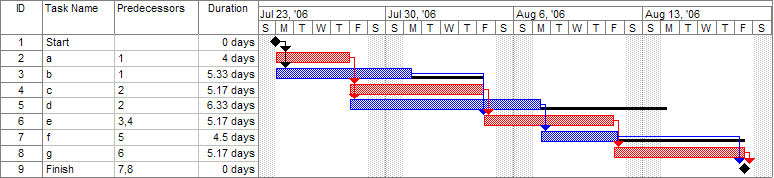
\includegraphics[width=0.95\textwidth]{ganttChart.png}
\end{center}

Поначалу диаграмма Гантта тоже делается без учета ресурсов, т.е. вы показываете только зависимости между задачами. Эта диаграмма очень часто используется, поскольку она крайне наглядная и ее можно рисовать где угодно. Например, часто для этого используют Excel/Google Spreadsheets. 

\begin{center}
    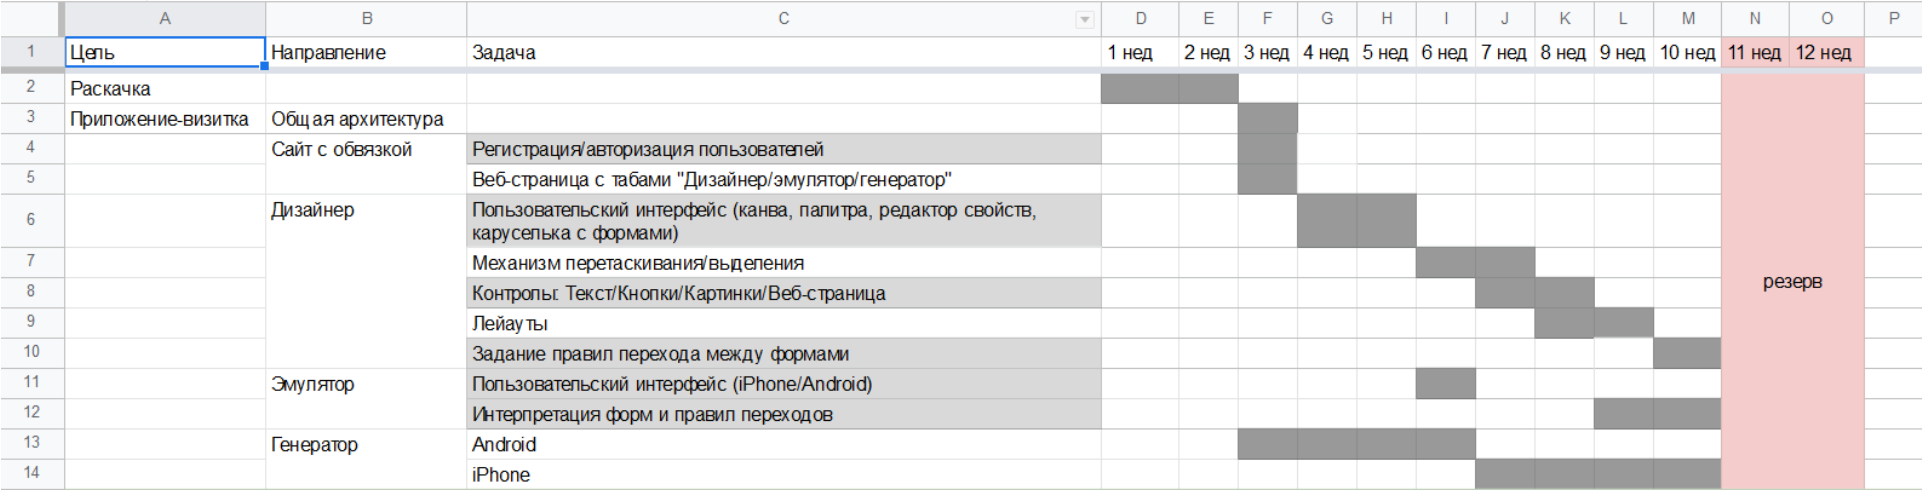
\includegraphics[width=0.95\textwidth]{ganttChartExample.png}
\end{center}

Единственная проблема, которая здесь будет~--- это перемещение задач. Т.е. если вы поняли, что вы сначала сделали задачу 4, а потом задачу 3, то просто поменять строки местами не получится. Вам еще потом придется сдвигать закрашенные ячейки.

\subsection{Диаграмма Гантта с указанием ресурсов}

\begin{center}
    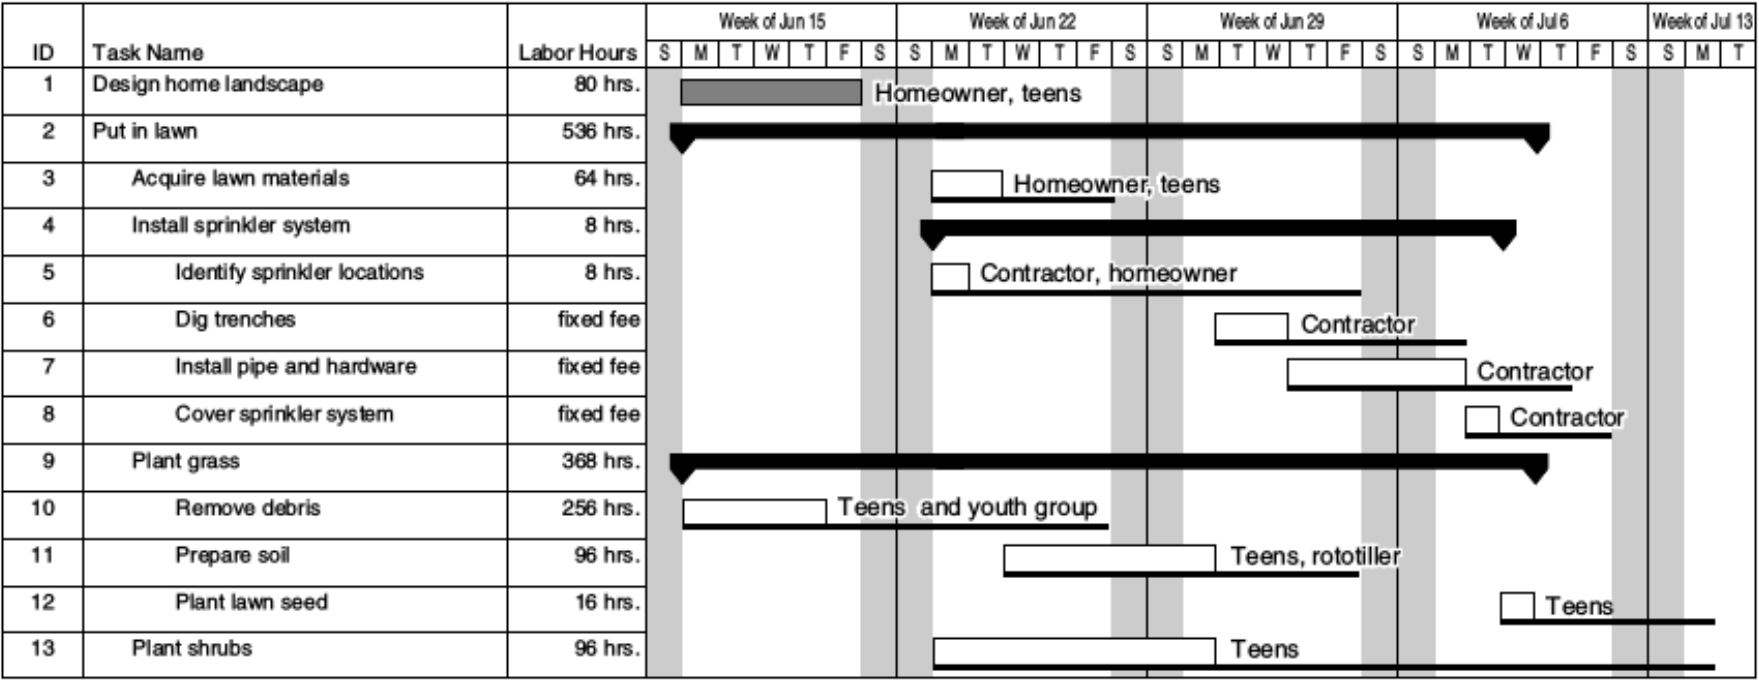
\includegraphics[width=0.95\textwidth]{ganttChartWithResources.png}
\end{center}

\begin{center}
    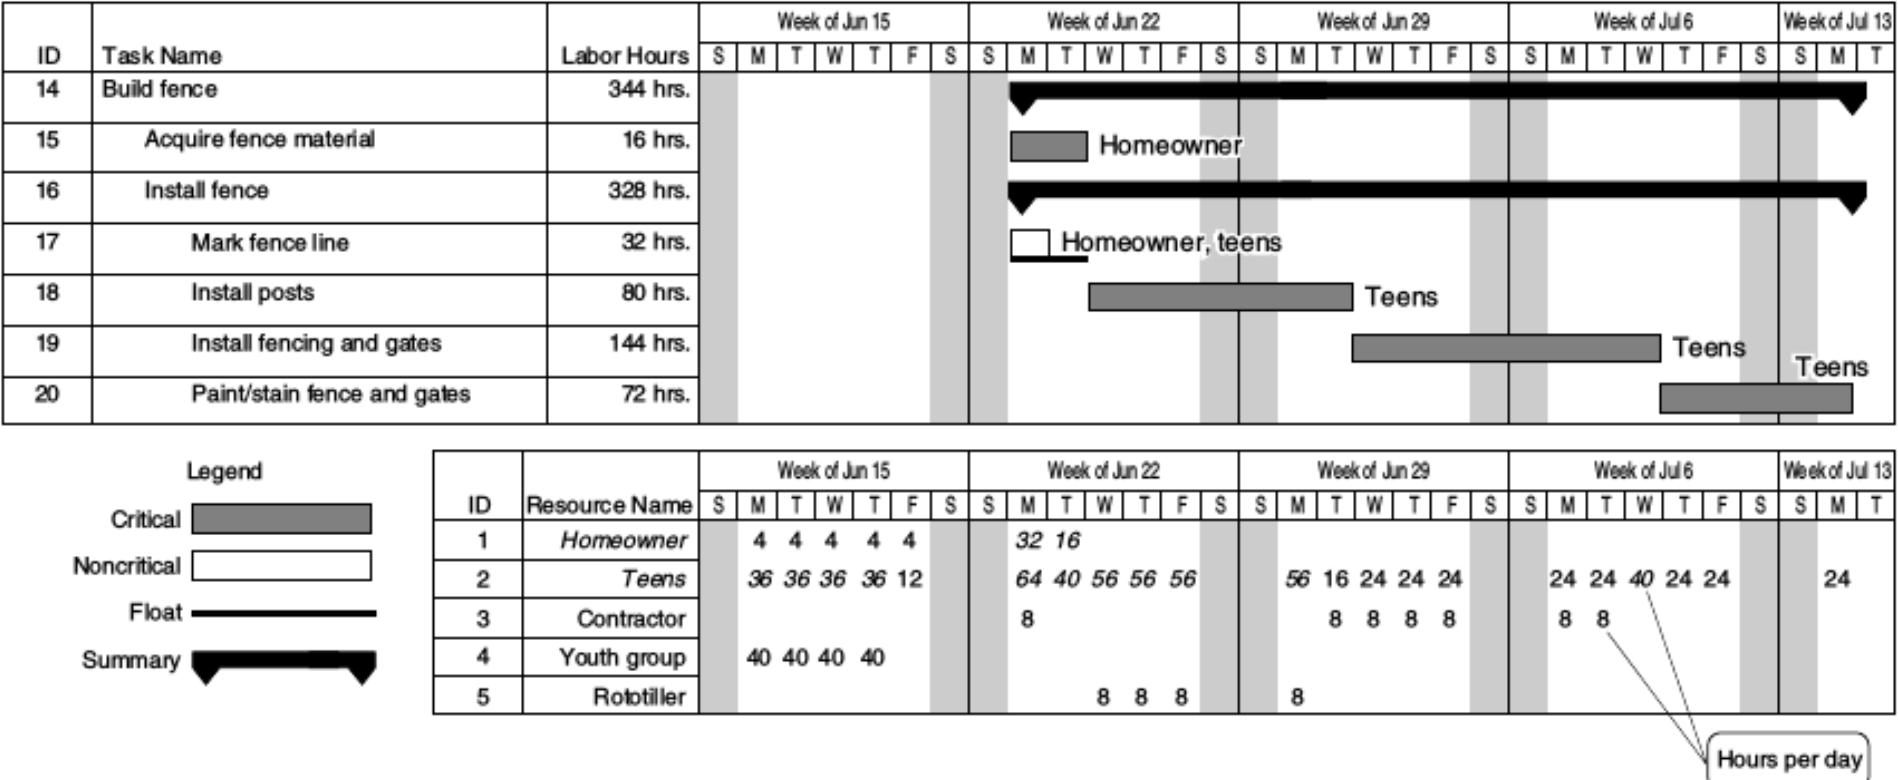
\includegraphics[width=0.95\textwidth]{ganttChartResourceUtilization.png}
\end{center}

На этой диаграмме еще указывается дополнительная информация. Здесь указаны составные задачи проекта (такие как \enquote{Put in lawn}), т.е. задачи, которые разбиваются на несколько других (промежуточный узел дерева декомпозиции). Жирной чёрной линией указан резерв (например, у задачи \enquote{Remove debris}), но в целом указывать его не обязательно.

Также на обычной диаграмме Гантта вообще нет информации о людях. Т.е. не указывается, кто делает какую задачу. А здесь эти сведения добавляют. Такую диаграмму можно достаточно быстро читать и в ней закладывается довольно много информации.

\subsection{Оптимизация ресурсов}

Итак, вы построили начальный план. Он потому и начальный, что он в принципе не подразумевает никакого распределения ресурсов. Начальный план показывает то, как задача была бы сделана в идеальном случае, но такого почти никогда не бывает. Поэтому этот план нужно оптимизировать в соответствии с ресурсами, которыми вы располагаете. Ресурсы~--- это люди, оборудование, материалы и т.п.

Здесь есть два понятия: перегруженность (overallocation) и недозагруженность (underallocation). Перегруженность означает, что вы пытаетесь перегрузить ваши ресурсы работой. Например, у вас есть один программист и вы ему нарисовали диаграмму, где он должен параллельно заниматься пятью задачами. Разумеется, он за один день не сделает 5 задач, длительность каждой из которых составляет один день. Он будет делать их 5 дней, и ваш график поедет. Перегруженность плоха ещё и потому, что когда вы перегружаете человека, он быстро устаёт и переутомляется, у него падает производительность.

Другая сторона проблемы~--- это недозагруженность: ситуация, при которой есть люди, которые ничем не заняты. Понятно, что это тоже плохо, поскольку вы просто теряете деньги, плюс это почти всегда сказывается негативно на большинстве людей. Чаще всего программисты работают не за зарплату. Программисты хотят решать интересные задачи, и в отсутствии достойной работы им реально становится скучно. Хорошие программисты долго на таких местах обычно не задерживаются. А в некоторых странах вот даже такое бывает: \url{https://www.personneltoday.com/hr/interparfums-boreout-case/} (дата обращения: 26.03.2025г).

Смотря на самую последнюю версию диаграммы Гантта, вы можете построить следующий график:

\begin{center}
    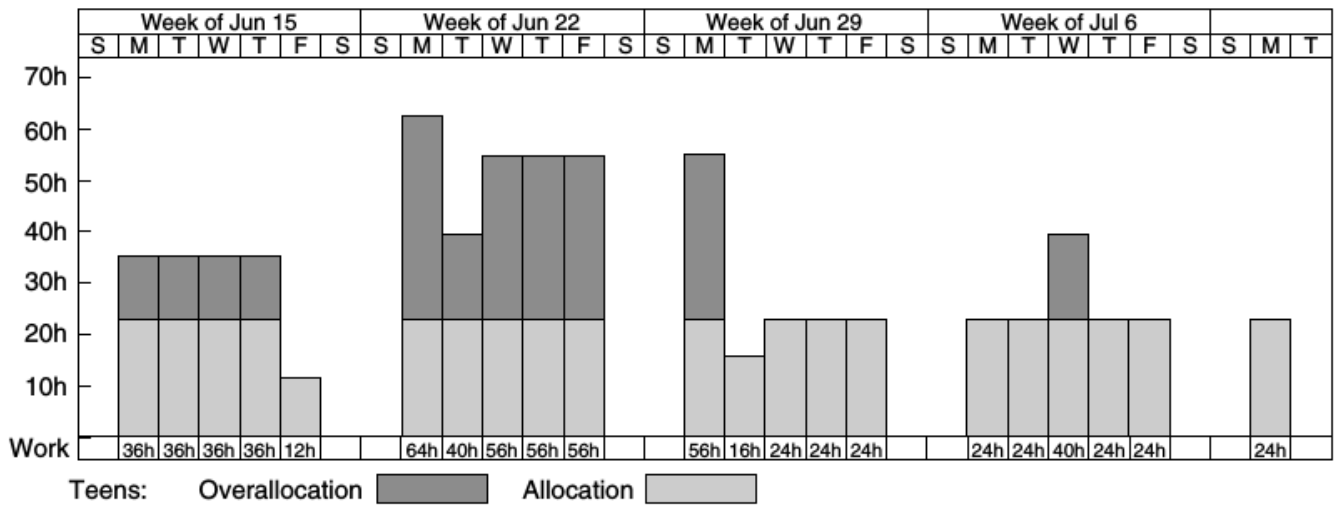
\includegraphics[width=0.7\textwidth]{resourceAllocation.png}
\end{center}

Видно, что в первый день вам нужно 36 человеко-часов, во второй 36 ч/ч, а в пятый 12 ч/ч. Человек в день должен работать по 8 часов, не более. В предыдущей таблице было три разработчика. Поэтому здесь allocation отмечено как 24 ч/ч~--- сколько они в сумме могут отработать за один день. Это пример несбалансированного графика работ.

Глядя на такие диаграммы, вы понимаете, что у вас есть пики (когда вы пытаетесь сделать слишком много), их имеет смысл выравнивать. Чтобы этого добиться, вы просто пытаетесь двигать ваши задачи в соответствии с тем резервом, который у них есть. Если у некоторой задачи резерв равен 9, то вы ее можете двигать в пределах девяти единиц времени. Вы можете отложить ее на 9, но она все равно не повлияет на конечный дедлайн. Т.е. резерв вам позволяет перемещать эти задачи по времени. В нашем примере, надо сдвигать задачи с первых четырёх дней на пятый. В этом примере это всё равно не позволит загрузить всех равномерно и сделать всё вовремя, но как первый шаг это вполне стоит того. Далее, если время является ключевым фактором, нужно искать возможность добавить людей на критические задачи или как-то иначе выровнять график. Но это тоже не всегда просто сделать: программисты~--- не укладчики кирпичей, которых можно без проблем заменять одного на другого. В итоге получается жонглирование большим количеством параметров, к которому нужно подходить очень аккуратно.

\subsection{Типичные ошибки при оценке проектов}

Есть несколько распространённых ошибок при оценке проектов, про которые все знают, но тем не менее, которые все делают. Перечислим их.

\textbf{Оценку делали не те люди. Мало опыта, непонимание техник оценивания.} Оценки должны делать нужные люди. Важно, чтобы это были те люди, которые хорошо знают предметную область. Независимо от того, какие методы используются, оценка всегда основывается на понимании работы, которую предстоит выполнить. Также к оценке стоит привлекать людей, которые будут фактически выполнять эту работу. Они имеют лучшее понимание своих способностей, к тому же, если человек знает, что ему предстоит делать данную задачу, то он ответственнее подойдет к ее оценке. Но при этом, если у вас нет никакого опыта оценивания, то первую оценку, скорее всего, вы сделаете очень плохо. Со временем, если вы будете анализировать и использовать свой опыт, вы научитесь это делать более точно.

\textbf{Слишком быстрый ответ и оценка в условиях недостаточной информации.} Никогда не давайте быстрых ответов. Вы всегда что-нибудь забудете, всегда оцените более оптимистично, чем хотелось бы. Поэтому есть несколько стратегий, как с этим бороться.

\begin{itemize}
    \item Каким-то образом откажитесь от ответа, но это не всегда оказывается возможным.
    \item Начните задавать вопросы, уточнять некоторые моменты. Когда вы получите больше информации, вы сможете точнее сделать оценку. Но, скорее всего, информации у того человека, который вас это спрашивает, нет. Поэтому после несколько вопросов, на которые вам не смогли дать ответ, менеджер сам поймет, что слишком много неизвестных, чтобы дать сейчас точную оценку.
    \item Попробуйте оценить задачу максимально точно, а потом умножьте ее на два. А затем еще раз на два. Это тот коэффициент, который, скорее всего, будет похож на правду. Т.е. если вы про что-нибудь не знаете или забудете, то благодаря этому коэффициенту вы с большой долей вероятности все туда уложите.
\end{itemize}

\begin{center}
    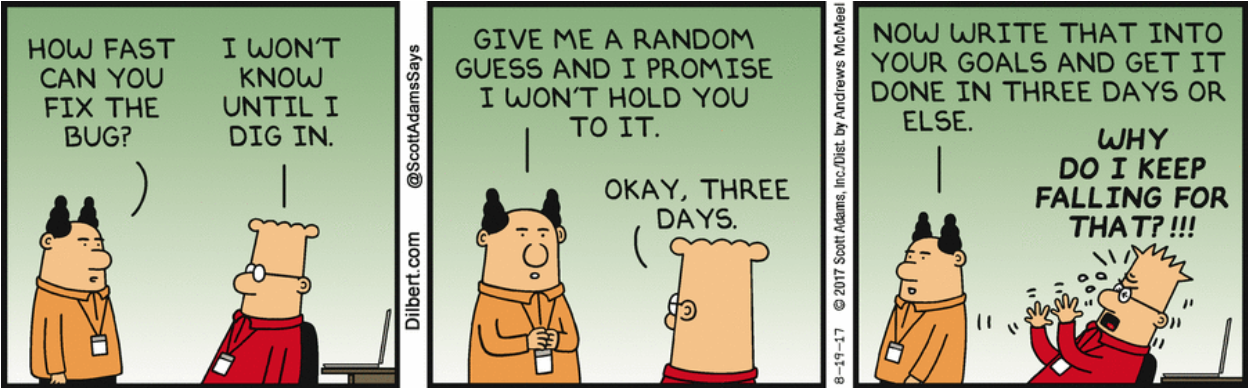
\includegraphics[width=0.7\textwidth]{dilbertEstimation.png}
\end{center}

\textbf{Забыли про риски и прочие буферы.} В начале лекции мы говорили о том, что противодействие рискам стоит денег. Скорее всего, если вы умножите вашу изначальную оценку на 4, то этот бюджет на риски и прочие буферы туда просто войдут автоматически, хотя бы частично. Но если вы этого не делаете, то проведите переоценку рисков, продумайте, как реализация и интеграция этой задачи повлияет на другие задачи и проект в целом.

\textbf{Забыли про налоги.} У вас есть диаграммы, вы посчитали количество человеко-часов, умножили их на зарплату. Допустим, что вы учли подоходный налог, но при этом забыли про все остальные налоги, половину бюджета вы просто выкинули. С человека государство берет 13\%, но с компании гораздо больше, до 54\%. Если это не заложить в бюджет, вам придется это платить из собственного кармана.

\textbf{Забыли про расходы на \enquote{административный аппарат}.} Еще один пункт, который включается в общую сумму проекта. Вы считаете затраты по задачам, которые делают программисты. Вы учитываете их зарплаты, подсчитываете общий бюджет, свою зарплату вы тоже скорее всего посчитали. Но есть еще уборщица, водитель, отдел кадров, менеджеры над вами, бухгалтеры, ген. директор, его секретарь и т.д. Назовем их \enquote{административным аппаратом}, и им тоже нужно платить деньги. Поэтому вы должны добавить к общей сумме проекта еще некий процент на эти издержки. Если у вас компания маленькая (10–20 чел), то процент будет небольшой (5–10\%). Если у вас компания побольше (300–400 чел), то накрутка может доходить до 30–40\%. И заказчики платят эти деньги, потому что крупная компания считается более надёжной, не совершает \enquote{детских ошибок} и т.п.

\textbf{Забыли про отпуск.} Вы берете ваш график и рассчитываете для каждого человека: 8ч в день => 40ч в неделю => x часов в год. Но потом оказывается, что работа у вас вовремя не заканчивается, поскольку 1/12 вы куда-то потеряли. Отпуск~--- это то время, когда человек освобождается от работы для отдыха. Причём не отправлять человека в отпуск нельзя, даже если он не против поработать~--- по закону хотя бы две недели отгулять обязательно.

\textbf{Забыли про индексацию зарплат.} Уровень жизни с каждым годом растет, цены в магазинах растут, зарплаты, соответственно, тоже понемногу увеличиваются. Если вы планируете долгий проект, который длится несколько лет, то необходимо учитывать, что зарплаты людей не будут стоять на месте. 

\textbf{Забыли про закупки.} Не учли деньги на приобретение разного рода товаров: компьютеры, столы, стулья, еда... Это, конечно, не такой большой бюджет, но про них не стоит забывать.

\textbf{Политика против здравого смысла.} Очень часто на менеджера происходит давление со стороны заказчика или собственного руководства, которые пытаются заставить его ужать как-нибудь график. Например, просит сделать так, чтобы проект закончился на 2 месяца быстрее или стоил на 10\% дешевле. Если вам нужно сделать на 10\% дешевле проект, уменьшайте задачи. Никогда нельзя идти на поводу: \enquote{давайте вы мне сделаете проект на 10\% дешевле, а я вам потом тоже что-нибудь хорошее сделаю}~--- так не работает. Вы ведь не просто так придумали этот график и стоимость. Вы так сделали, потому что есть объективные реальности. У вас эта оценка обоснованная, поэтому эти 10\% невозможно просто так выкинуть.

\subsection{Уровни детальности оценки}

Конечно, мы всегда хотим как можно более точных оценок, но точность стоит денег. Поэтому имеет смысл использовать различные методы оценки для различных точек принятия решения в проекте. Например, первоначальная оценка идеи проекта не должна занимать столько времени и усилий, сколько детальное планирование, необходимое для официального проекта.

Есть три уровня детальности оценки.

\begin{enumerate}
    \item Неточная оценка, которую вы даете, особо не задумываясь. Она нужна на самом раннем уровне, когда вы просто пытаетесь понять, насколько это большой, масштабный и сложный проект.
    \item Второй уровень~--- это когда вы несколько часов посидели и подумали. Вы не делаете подробную декомпозицию, но вы уже собрали какую-то информацию, что-то порисовали на листочке. Обычно на основе этой второй оценки принимается решение: идти дальше или нет. Т.е. здесь вы уже прикидываете: оправдает ли результат затраченные средства? Осуществим ли проект технически? Часто бывает так, что ожидания заказчика по стоимости проекта или его способность платить меньше, чем вам необходимо, чтобы даже покрыть все перечисленные выше расходы, не говоря уже о получении значимого процента прибыли, которую от вас ожидает руководство. Или в продуктовых проектах оцениваемый объём рынка может быть меньше, чем затраты на разработку, так что даже если 100\% вашей целевой аудитории купят ваш продукт (что не бывает), вы всё равно окажетесь в минусе. В таких случаях проект заканчивается тут же, даже не начавшись.
    \item Если вы дважды сказали себе \enquote{да}, значит, вы готовы продолжить и взяться за проект. Дальше делается детальная оценка. Она включает в себя всю информацию о графике и ресурсах. Это оценка будет использоваться для управления проектом и оценки его успеха. Чтобы сделать подробную декомпозицию большого проекта, вам может потребоваться несколько недель.
\end{enumerate}

В зависимости от стадии проекта, необходимой степени точности, возможных расходов и трудозатрат применяются различные типы оценок стоимости:
\begin{itemize}
    \item Метод оценки \enquote{сверху-вниз} используется для определения затрат на ранних стадиях проекта, когда информации о проекте еще очень мало. Смысл такой оценки в том, что она производится обобщенно и проект оценивается в целом. Сначала дается укрупненная оценка всего пакета работ, а затем она детализируется и декомпозируется на отдельные элементы, которые, в свою очередь, также оцениваются.
    \item Метод оценки \enquote{снизу-вверх} нужен для выработки согласованной базовой цены проекта или окончательной стоимостной оценки проекта. Название метода отражает способ расчета стоимостной оценки~--- данный подход предусматривает оценку затрат на детальных уровнях проекта с последующим суммированием элементов на более высоких уровнях.
\end{itemize}

\subsection{Планирование денежных потоков}

Одной из главных проблем любого бизнеса является правильное планирование денежных потоков. Даже рентабельные предприятия терпят банкротство из-за нехватки денежных поступлений. Нельзя только по уровню прибыли судить о мере финансовой устойчивости компании~--- например, у вас есть заказчик, который в декабре переведёт вам N рублей, но сейчас сентябрь, на счету закончились деньги, кредитные лимиты исчерпаны, и надо платить разработчикам n (много меньше, чем N) рублей. Вы задерживаете зарплату, один из сотрудников подаёт иск, компания банкротится, активы распродаются, зарплата выплачивается из доходов от продажи активов. N рублей остаётся на счету заказчика, поскольку юрлицо ликвидировано и деньги перевести уже некуда. А если суд усмотрит корыстный интерес гендиректора в задержке зарплаты, это уже может быть тюремный срок.

Управление денежными потоками~--- это одна из наиболее важных задач финансового менеджмента. Для обеспечения платежеспособности компании и выполнения всех финансовых обязательств необходимо рациональное распределение и управление денежными потоками в организации. Необходимо спланировать синхронность поступления и расходования денежных средств и таким образом поддержать текущую платежеспособность предприятия.

\begin{center}
    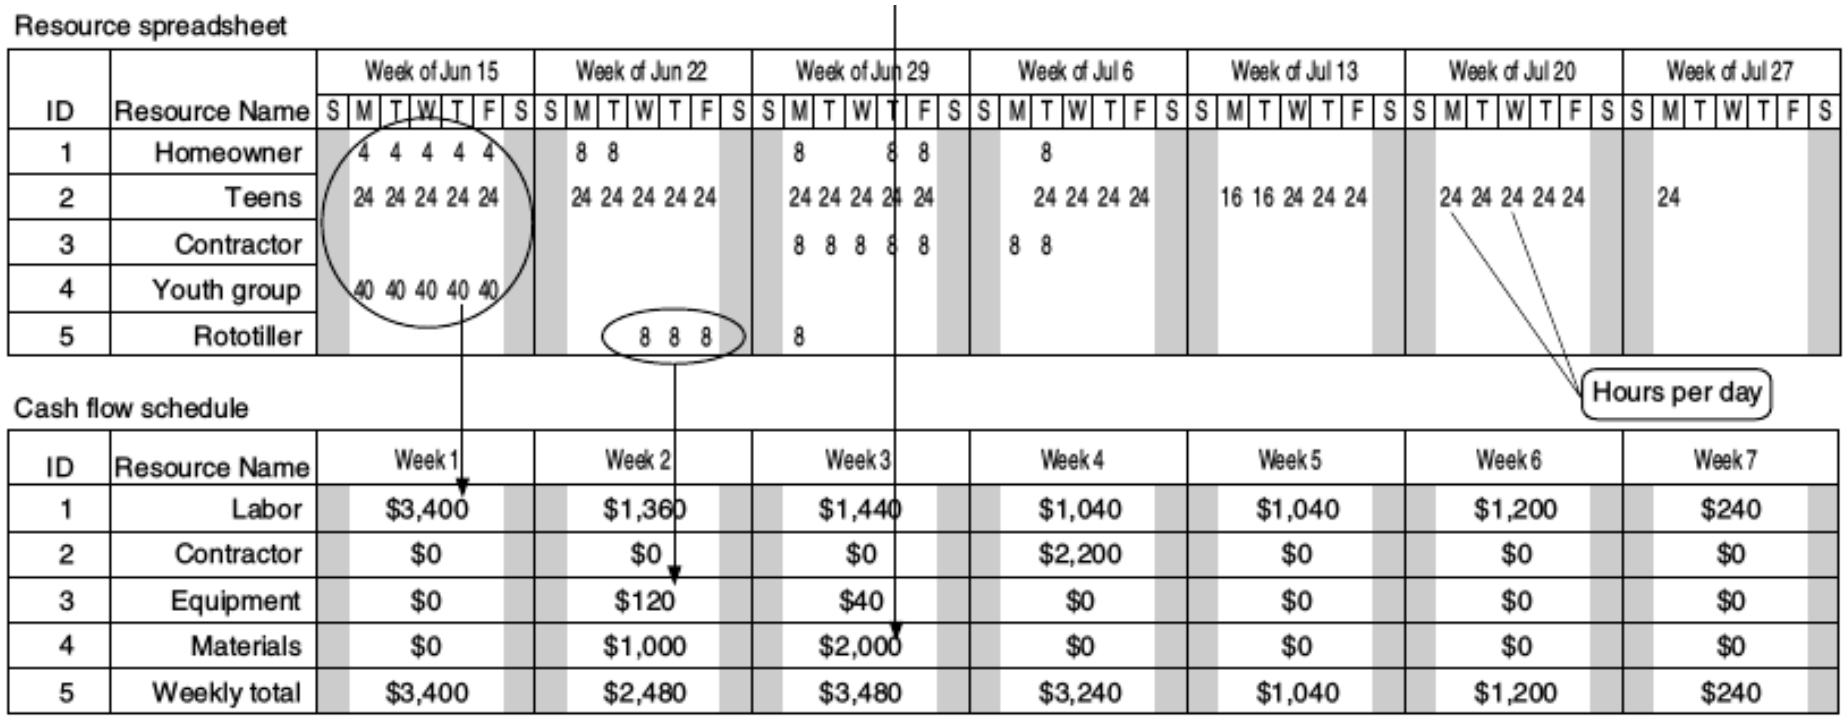
\includegraphics[width=0.95\textwidth]{cashFlow.png}
\end{center}

При планировании денежных потоков вы определяете, когда и сколько денег поступит или будет уплачено по счетам, чтобы обеспечить нормальную деятельность предприятия. При этом необходимо учесть возможный временной сдвиг между реальным заключением договора и фактическим получением денег. В начале проекта вы скорее всего получите лишь небольшой аванс, а остальные деньги будете получать частями по достижении заранее оговоренных ключевых точек, либо, в худшем случае, в самом конце, когда проект будет завершён. Ну и надо понимать, что банковский перевод от заказчика к вам и от вас к сотрудникам тоже занимает время, а зарплату вы обязаны платить в оговоренные сроки.

\end{document}
